\documentclass[12pt,letter paper]{article}
\usepackage{siunitx}
\usepackage{setspace}
\usepackage{gensymb}
\usepackage{xcolor}
\usepackage{caption}
%\usepackage{subcaption}
\doublespacing
\singlespacing
\usepackage[none]{hyphenat}
\usepackage{amssymb}
\usepackage{relsize}
\usepackage[cmex10]{amsmath}
\usepackage{mathtools}
\usepackage{amsmath}
\usepackage{commath}
\usepackage{amsthm}
\interdisplaylinepenalty=2500
%\savesymbol{iint}
\usepackage{txfonts}
%\restoresymbol{TXF}{iint}
\usepackage{wasysym}
\usepackage{amsthm}
\usepackage{mathrsfs}
\usepackage{txfonts}
\let\vec\mathbf{}
\usepackage{stfloats}
\usepackage{float}
\usepackage{cite}
\usepackage{cases}
\usepackage{subfig}
%\usepackage{xtab}
\usepackage{longtable}
\usepackage{multirow}
%\usepackage{algorithm}
\usepackage{amssymb}
%\usepackage{algpseudocode}
\usepackage{enumitem}
\usepackage{mathtools}
%\usepackage{eenrc}
%\usepackage[framemethod=tikz]{mdframed}
\usepackage{listings}
%\usepackage{listings}
\usepackage[latin1]{inputenc}
%%\usepackage{color}{   
%%\usepackage{lscape}
\usepackage{textcomp}
\usepackage{titling}
\usepackage{hyperref}
%\usepackage{fulbigskip}   
\usepackage{tikz}
\usepackage{graphicx}
\lstset{
  frame=single,
  breaklines=true
}
\let\vec\mathbf{}
\usepackage{enumitem}
\usepackage{graphicx}
\usepackage{siunitx}
\let\vec\mathbf{}
\usepackage{enumitem}
\usepackage{graphicx}
\usepackage{enumitem}
\usepackage{tfrupee}
\usepackage{amsmath}
\usepackage{amssymb}
\usepackage{mwe} % for blindtext and example-image-a in example
\usepackage{wrapfig}
\graphicspath{{figs/}}
\providecommand{\mydet}[1]{\ensuremath{\begin{v\matrix}#1\end{v\matrix}}}
\providecommand{\myvec}[1]{\ensuremath{\begin{b\matrix}#1\end{b\matrix}}}
\providecommand{\cbrak}[1]{\ensuremath{\left\{#1\right\}}}
\providecommand{\brak}[1]{\ensuremath{\left(#1\right)}}
\providecommand{\sbrak}[1]{\ensuremath{{}\left[#1\right]}}
\title{Questions}
\date{}
\author{}
\begin{document}
\maketitle{}
\begin{center}
	\section*{Geometry}
\end{center}
\begin{enumerate}
    \item The dimensions of a solid iron cuboid are $4.4\,\mathrm{m} \times 2.6\,\mathrm{m} \times 1.0\,\mathrm{m}$. It is melted and recast into a hollow cylindrical pipe of $30\,\mathrm{cm}$ inner radius and thickness $5\,\mathrm{cm}$. Find the length of the pipe.
    \item Prove that the lengths of two tangents drawn from an external point to a circle are equal.
    \item In the given figure, $XY$ and $X'Y'$ are two parallel tangents to a circle with centre $O$ and another tangent $AB$ with point of contact $C$, is intersecting $XY$ at $A$ and $X'Y'$ at $B$. Prove that $\angle AOB = 90\degree$.
\begin{figure}[H]
\centering
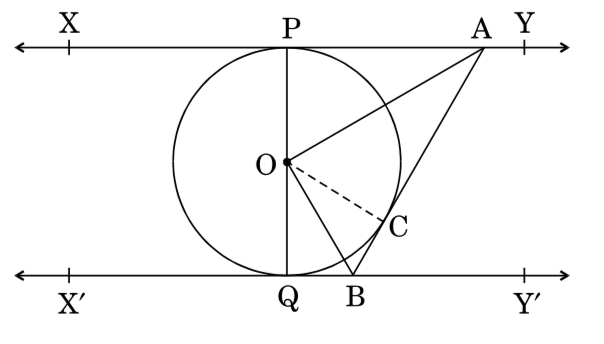
\includegraphics[width=\columnwidth]{fig1.jpg}
\caption{}
\end{figure}
    \item Construct a triangle $ABC$ with side $BC = 7\,\mathrm{cm}$, $\angle B = 45\degree$, $\angle A = 105\degree$. Then construct another triangle whose sides are $\frac{3}{4}$ times the corresponding sides of the $\triangle ABC$.
    \item If the points $A\brak{k + 1, 2k}$, $B\brak{3k, 2k + 3}$ and $C\brak{5k - 1, 5k}$ are collinear, then find the value of $k$.
    \item In the given figure,$ABCD$ is a rectangle of dimensions $21\,\mathrm{cm} \times 14\,\mathrm{cm}$. A semicircle is drawn with $BC$ as diameter. Find the area and the perimeter of the shaded region in the figure.
\begin{figure}[H]
\centering                          
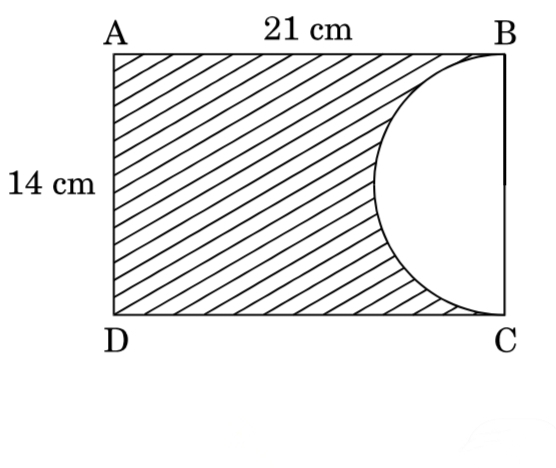
\includegraphics[width=\columnwidth]{fig2.jpg}
\caption{}
\end{figure}
\item In a rain-water harvesting system, the rain-water from a roof of $22\,\mathrm{m} \times 20\,\mathrm{m}$ drains into a cylindrical tank having diameter of base $2\,\mathrm{m}$ and height $3.5\,\mathrm{m}$. If the tank is full, find the rainfall in $\mathrm{cm}$. Write your views on water conservation.
\end{enumerate}
\begin{center}
	\section*{Algebraic equations}
\end{center}
\begin{enumerate}
\item Solve for $x$:
$\frac{1}{x+1} + \frac{3}{5x+1} = \frac{5}{x+4}, \quad x \neq -1, -\frac{1}{5},-4$
\end{enumerate}
\begin{center}
	\section*{Work and Time}
\end{center}
\begin{enumerate}
    \item Two taps running together can fill a tank in $3\frac{1}{13}$ hours. If one tap takes $3$ hours more than the other to fill the tank, then how much time will each tap take to fill the tank?
\end{enumerate}
\begin{center}
	\section*{Sequence and Series}
\end{center}
\begin{enumerate}
	\item If the ratio of the sum of the first $n$ terms of two A.Ps is $\brak{7n + 1} : \brak{4n + 27}$, then find the ratio of their $9^{th}$ terms.
\end{enumerate}
\begin{center}
	\section*{Trigonometry}
\end{center}
\begin{enumerate}
	\item An aeroplane is flying at a height of $300\,\mathrm{m}$ above the ground. Flying at this height, the angles of depression from the aeroplane of two points on both banks of a river in opposite directions are $45\degree$ and $60\degree$ respectively. Find the width of the river.
		$\sbrak{Use \sqrt{3}=1.732}$
\end{enumerate}
\begin{center}
	\section*{Probability}
\end{center}
\begin{enumerate}
\item Two different dice are thrown together. Find the probability that the numbers obtained have
     \begin{enumerate}
        \item an even sum, and
        \item an even product.
    \end{enumerate}
\end{enumerate}
\end{document}
